\documentclass[slovene,11pt,a4paper]{article}
%\usepackage{fullpage}
\usepackage[margin=2cm]{geometry}

\usepackage[T1]{fontenc}



%dodatni paketki:
\usepackage{graphicx}
\usepackage{amsmath,amsfonts,amsthm} %matematicni paket
\usepackage{color} % omogoča barvno pisanje
\usepackage[utf8]
{inputenc}
\usepackage[slovene]{babel} % slovenski jezik/hyphenation
\usepackage{hyperref} %naredi vse povezave rečerenc, kazala,...
\numberwithin{equation}{section} % Number equations within sections (i.e. 1.1, 1.2, 2.1, 2.2 instead of 1, 2, 3, 4)
\numberwithin{figure}{section} % Number figures within sections (i.e. 1.1, 1.2, 2.1, 2.2 instead of 1, 2, 3, 4)
\numberwithin{table}{section} % Number tables within sections (i.e. 1.1, 1.2, 2.1, 2.2 instead of 1, 2, 3, 4)
\usepackage{eurosym} %za znak €

\usepackage{mathrsfs}
\usepackage{mathabx} % za kemisjke smeri in naslednje 3 vstrice
\catcode`_=12
\begingroup\lccode`~=`_\lowercase{\endgroup\let~\sb}
\mathcode`_="8000


\usepackage[margin=2cm]{geometry}



\begin{document}
\begin{titlepage}

\newcommand{\HRule}{\rule{\linewidth}{0.5mm}} % Defines a new command for the horizontal lines, change thickness here

\center % Center everything on the page

%----------------------------------------------------------------------------------------
%	LOGO
%----------------------------------------------------------------------------------------

%\includegraphics{Logo}\\[1cm] % Include a department/university logo - this will require the graphicx package
 
%----------------------------------------------------------------------------------------


\includegraphics[width=2cm]{slike/aaa}\\[0.5cm]
 
%----------------------------------------------------------------------------------------
%	NASLOV DELA
%----------------------------------------------------------------------------------------
\textit{Univerza v Ljubljani}\\
\textit{Fakulteta za {\color{red}matematiko in fiziko}}\\[0.5cm]

\emph{Oddelek za fiziko}\\[0.5cm] % Oddelek za fiziko


%----------------------------------------------------------------------------------------
%	TITLE SECTION
%--------------------------------------------------------------------------------------
\HRule \\[0.4cm]
\huge {\bfseries 8. naloga: - Generatorji naključnih števil}\\[0.4cm] % NASLOV SEMINARJA
\HRule \\[0.5cm] 

 \textsc{\large Poročilo pri predmetu modelska analiza 1}\\
 \textsc{\large 2015/2016}\\[1cm] % SEMINASKO DELO
 
%----------------------------------------------------------------------------------------
%	AUTHOR SECTION
%----------------------------------------------------------------------------------------



% If you don't want a supervisor, uncomment the two lines below and remove the section above
\Large \emph{Avtor:}\\
Klemen \textsc{Rahne}\\
28152028\\[2cm]
%----------------------------------------------------------------------------------------
%	DATUM
%----------------------------------------------------------------------------------------

{\large \today } \\[0.5cm] % Date, change the \today to a set date if you want to be precise

	

\end{titlepage}


%----------------------------------------------------------------------------------------
%	KAZALO
%----------------------------------------------------------------------------------------

%\tableofcontents

%----------------------------------------------------------------------------------------
%	ZAČETEK TEKSTA
%----------------------------------------------------------------------------------------
\section{Teorija-uvod}
V tokratni nalogi bomo preverjali generatorje naključnih števil. Generatorje bomo preverili s testom Kolmogorov-Smirnova ter testom $\chi^2$.

\subsection{Test $\chi^2$}

Pri testiranju porazdelitve števil v testu $\chi^2$, najprej razpon števk razdelimo v $m$ predalov. V $i-tem$ predalčku je torej $N_i$ števk, oz. verjetnost da posamezna števka pade v $i-ti$ predalček je $\rho' =\frac{N_k}{n}$, kjer je $n$ število vseh števk. Pri vsakem testu moramo tudi predpostaviti analitično porazdelitev. Analitična verjetnost, da pade števka v $i-ti$ predalček je:
\begin{equation}
\rho_i = \int_{x_i}^{x_{i+1}} \frac{dP}{dx} dx
\end{equation}
kjer je $\frac{dP}{dx}$ analitična porazdelitev, $x_i, x_{i+1}$, spodnja in zgornja meja predala. Test $\chi^2$:

\begin{equation}
\chi^2 =\sum_{i=1}^m  \frac{ ( N_i - \rho_i n)^2 }{ n \rho_i } 
\end{equation}
Ker imamo veliko število $n$, je v limiti $\chi^2$ porazdeljen neodvisno od porazdelitve $\frac{dP}{dx}$:
\begin{equation}
\frac{d P}{d \chi^2}= \frac{1}{2^{\frac{m-1}{2}} \Gamma(m-\frac{1}{2})} (\chi^2)^{\frac{m-3}{2}} e^{-\frac{\chi^2}{2}}
\end{equation}	
Lahko določimo tudi zgornjo mejo $\chi^2_>$, ki na stopnjo tveganja $\alpha$ dovoljuje testni $\chi^2$:
\begin{equation}
\label{enacba-chi}
\int_{\chi^2_>}^{\infty} \frac{d P}{d \chi^2} d\chi^2 = \alpha
\end{equation}
Vrednosti $\chi^2_>$ za posamezno stopnjo tveganja $\alpha$ so že tabelirane.

\subsection{Test Kolmogorov-Smirnov}
Prav tako test Kolmogorov-Smirnov testira izmerjeno porazdelitev z analitično. Tokrat je potrebno imeti obe porazdelitve v kumulativni obliki:
\begin{equation}
\begin{aligned}
F(x)&=\int_{- \infty}^{x} \frac{d P}{d x} dx \\
F_i&=\frac{N_i}{N}
\end{aligned}
\end{equation}
kjer je $N_i$ število vseh števk v porazdelitvi manjših od $x_i$, katera je zgornja meja $i-tega$ predalčka. $N$ je število vseh števk v porazdelitvi. Pri testu Kolmogorov-Smirnov testiramo vrednost:
\begin{equation}
D=\sup|F_i-F(x_i)|
\end{equation}
ki predstavlja največje odstopanje testne kumulativne porazdelitve od analitične porazdelitve. 
Ponovno je $D$ porazdeljen ter lahko ponovno na stopnji tveganja $\alpha$ določimo zgornjo vrednost $D_>$:
\begin{equation}
\label{enacba-ks}
\lim_{n \rightarrow \infty} P(D \sqrt{N} < D_>) = \sum_{k=-\infty}^{\infty}(-1)^{k}e^{-2k^{2}D_>^{2}}=1-\alpha
\end{equation}
Tudi vrednosti $D_>$ so tabelirane.


\section{Generatorji enakomerno porazdeljenih števil}
Oglejmo si generator naključnih števil. Primerjali bomo dva generatorja. Prvi bo vgrajeni generator naključnih števil v programskem jeziku \textit{Python}, ki je osnovan na algoritmu Mersenne Twister. Drugi generator je linearni kongruenčni generator, z $a=1103515245$, $b=123454$ in $m=2^{32}$.

\begin{figure}[h]
\begin{center}
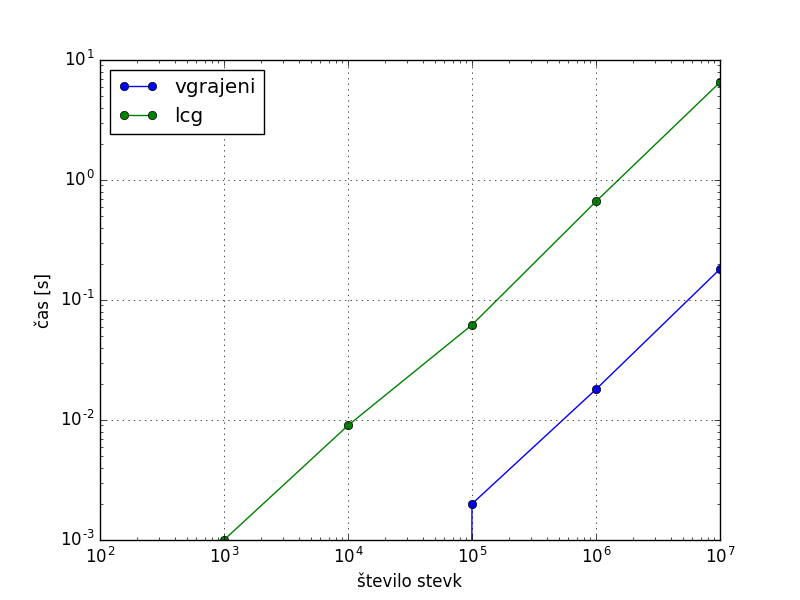
\includegraphics[scale=0.4]{slike/casovna_odvisnost.png}
\end{center}
\caption{Primerjava hitrosti testiranih generatorjev. Opazimo, da z naraščanjem potrebnih naključnih števil, skupni čas narašča linearno oz. za eno naključno številko potrebujemo enako časa, neodvisno od števila potrebnih številk. Opazimo, da je vgrajeni za več kot en velikostni razred hitrejši od linearnega. To je verjetno posledica tega, ker smo vgrajeni generator klicali iz knjižnice \textit{Numpy}, katera je specializirana za matematične operacije. Funkcijo za linearni kongruenčni generator sem napisal sam.}
\end{figure}

\begin{figure}[h]
\centering
\begin{minipage}{0.5\textwidth}
\centering
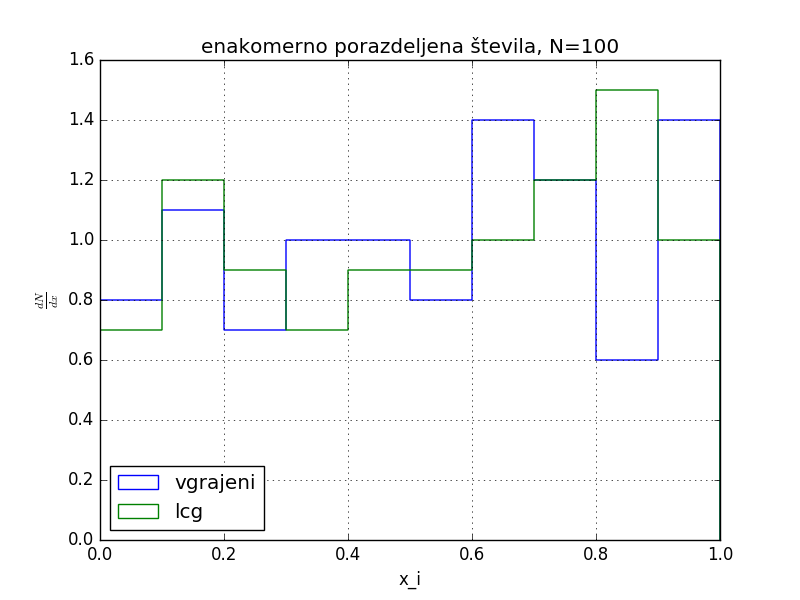
\includegraphics[scale=0.4]{slike/enakomerna_porazdelitev_N100.png}
%\caption{first figure}
\end{minipage}\hfill
\begin{minipage}{0.5\textwidth}
\centering
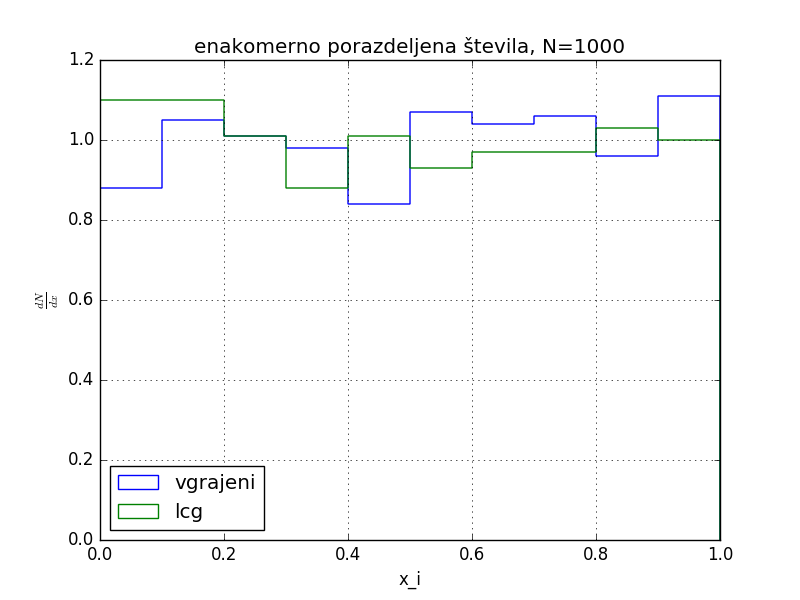
\includegraphics[scale=0.4]{slike/enakomerna_porazdelitev_N1000.png}
%\caption{second figure}
\end{minipage}
\begin{minipage}{0.5\textwidth}
\centering
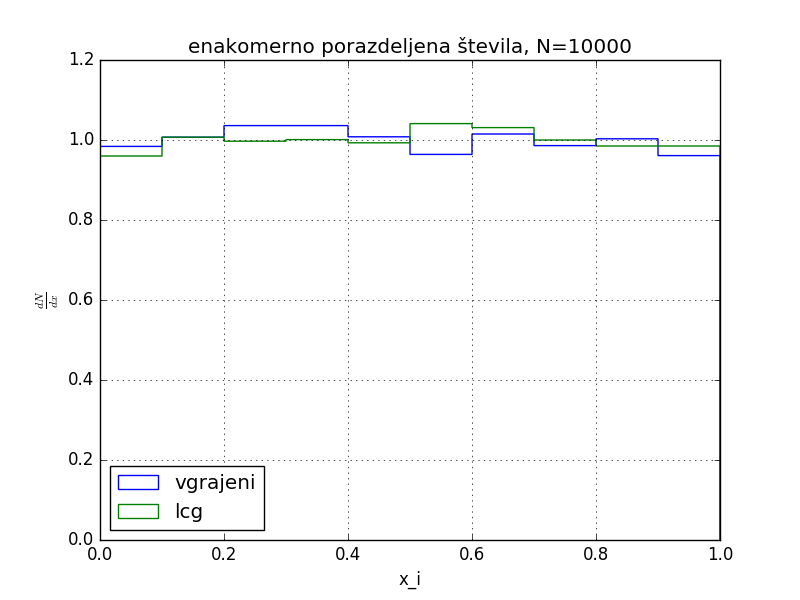
\includegraphics[scale=0.4]{slike/enakomerna_porazdelitev_N10000.png}
%\caption{first figure}
\end{minipage}\hfill

\caption{Primerjava dveh generatorjev naključnih števil. Na prvi pogled ne moremo oceniti, njune pravilnosti/napačnosti delovanja. Opazimo, da z naraščanjem števila $N$, se porazdelitev bliža analitični vrednosti, ki je $1$.}
\end{figure}



\clearpage



\subsection{Test $\chi^2$}
Testirajmo sedaj zgornja generatorja s testom $\chi^2$ in poglejmo njune porazdelitve vrednosti $\chi^2$.


\begin{figure}[h]
\centering
\begin{minipage}{0.4\textwidth}
\centering
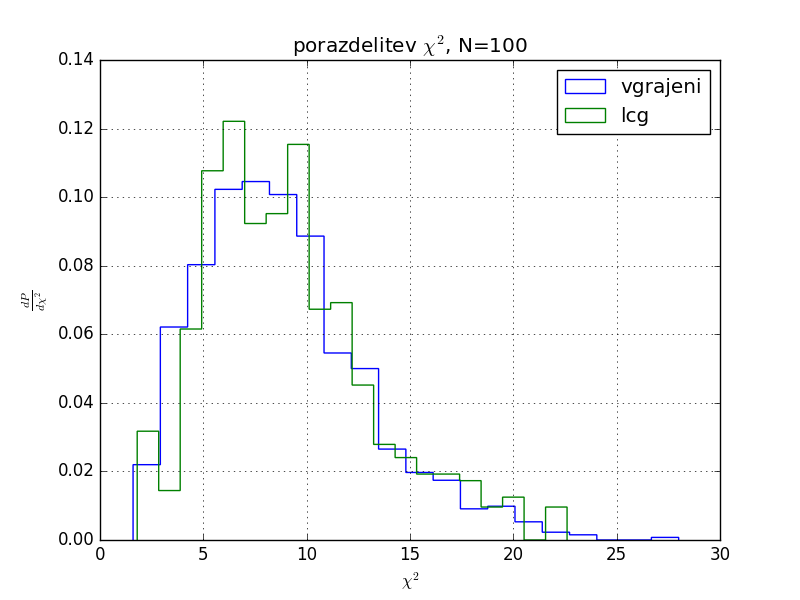
\includegraphics[scale=0.4]{slike/potazdelitev_chi_N_100.png}
%\caption{first figure}
\end{minipage}\hfill
\begin{minipage}{0.4\textwidth}
\centering
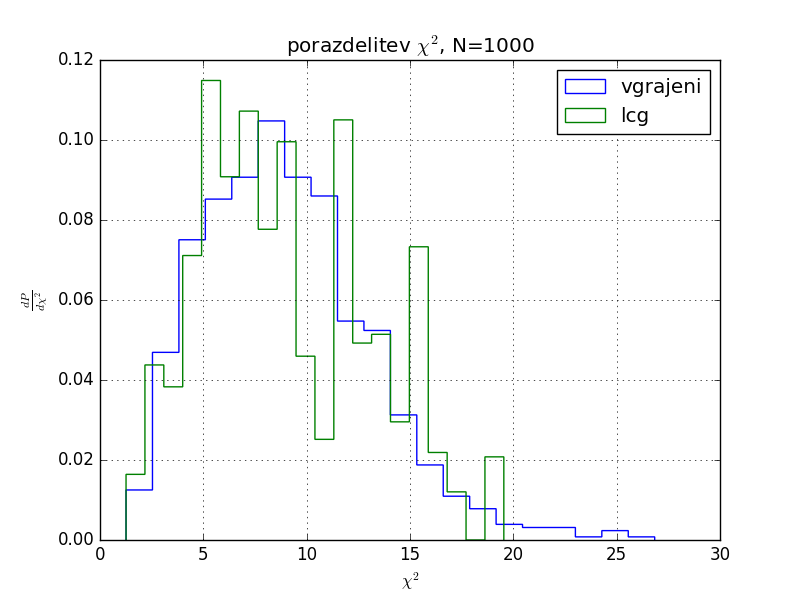
\includegraphics[scale=0.4]{slike/potazdelitev_chi_N_1000.png}
%\caption{second figure}
\end{minipage}
\begin{minipage}{0.4\textwidth}
\centering
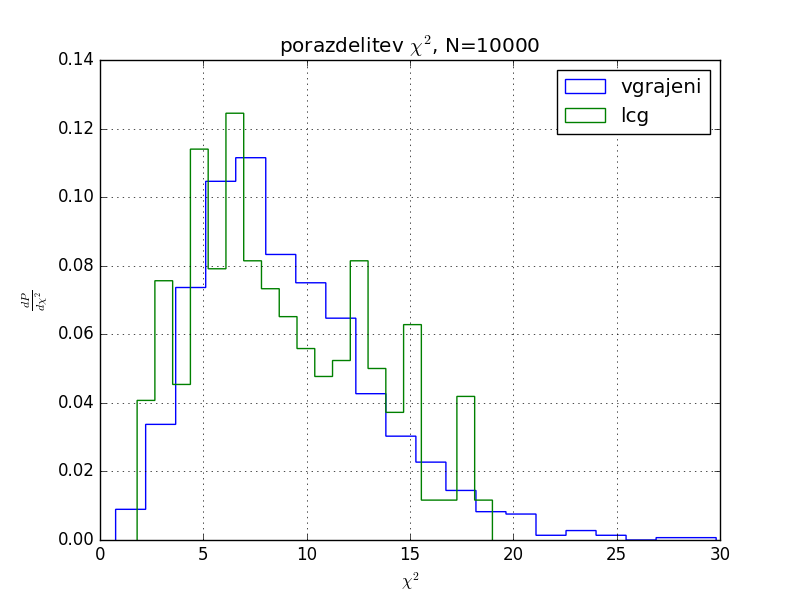
\includegraphics[scale=0.4]{slike/potazdelitev_chi_N_10000.png}
%\caption{first figure}
\end{minipage}\hfill

\caption{Porazdelitev $\chi^2$ obeh generatorjev v odvisnosti od števila generiranih številk. Oblike sta podobni, le da \textit{lcg} generator ima nekoliko večjo variacijo, od idealne zvezne porazdelitve. }
\end{figure}
Primerjajmo to porazdelitev še številčno. Iz enačbe \ref{enacba-chi} in njenih vrednosti lahko primerjamo naša generatorja naključnih števil. Za enakomerno porazdeljena števila so pričakovane vrednosti $\chi^2$:

\begin{table}[!h]
\begin{center}
\begin{tabular}{|l|l|l|l|}
\hline
stopnja tveganja $\alpha$ & $0.01$ & $0.5$ & $0.99$ \\ \hline
$m=9, \chi^2:$ & $21.67$ & $8.34$ & $2.09$ \\ \hline
\end{tabular}
\end{center}
\end{table}


\begin{table}[!h]
\begin{center}
\begin{tabular}{|l|l|l|l|l|}
\hline
generator & \multicolumn{2}{c|}{\textit{lcg}} &  \multicolumn{2}{c|}{vgrajeni}  \\ \hline
$N$ & povprečni $\chi^2$ & variacija $\chi^2$ & povprečni $\chi^2$ & variacija $\chi^2$ \\  \hline
$100$ & $9.05$ & $4.35$ & $9.34$ & $4.23$ \\ \hline
$1000$ & $9.18$ & $4.23$ & $9.04$ & $4.09$ \\ \hline
$10000$ & $9.17$ & $4.41$ & $9.05$ & $4.27$ \\ \hline
\end{tabular}
\end{center}
\caption{Izmerjene vrednosti $\chi^2$. Med generatorjema ni opaznih razlik v tem testu. Oba generatorja imata povprečno vrednost, ki je v okolici mejne vrednosti za $\alpha=50\%$. Potrebno pa je tudi opozoriti na zelo veliko varianco vrednosti $\chi^2$. }
\end{table}

\newpage
\subsection{Test Kolmogorov-Smirnov}



\begin{figure}[h]
\centering
\begin{minipage}{0.5\textwidth}
\centering
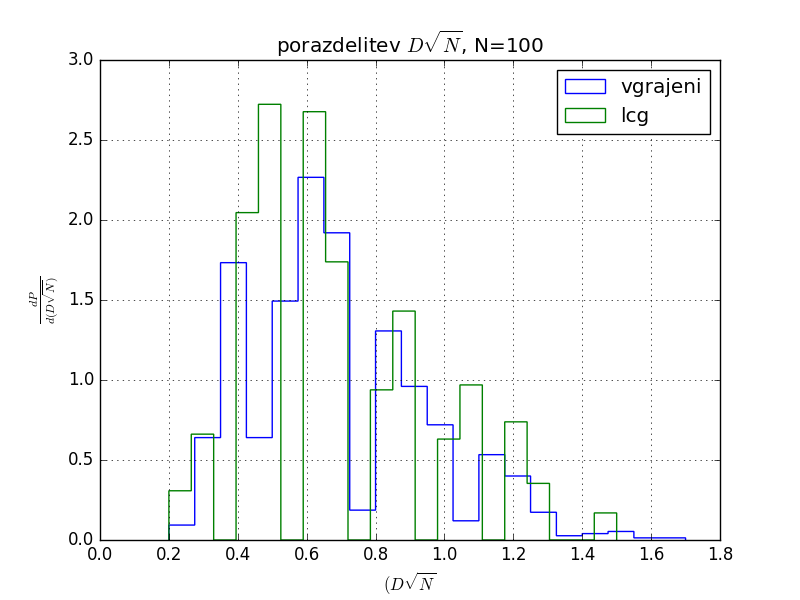
\includegraphics[scale=0.4]{slike/potazdelitev_DsqrtN_100.png}
%\caption{first figure}
\end{minipage}\hfill
\begin{minipage}{0.5\textwidth}
\centering
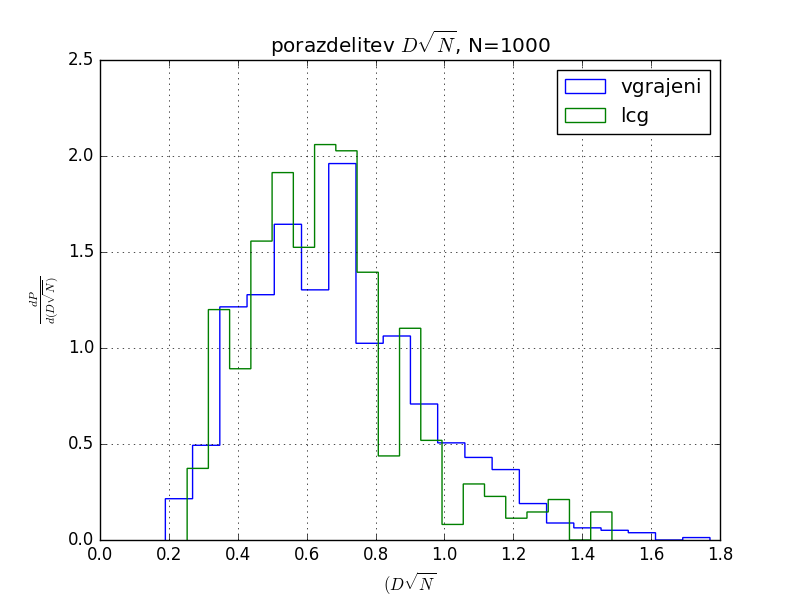
\includegraphics[scale=0.4]{slike/potazdelitev_DsqrtN_1000.png}
%\caption{second figure}
\end{minipage}
\begin{minipage}{0.5\textwidth}
\centering
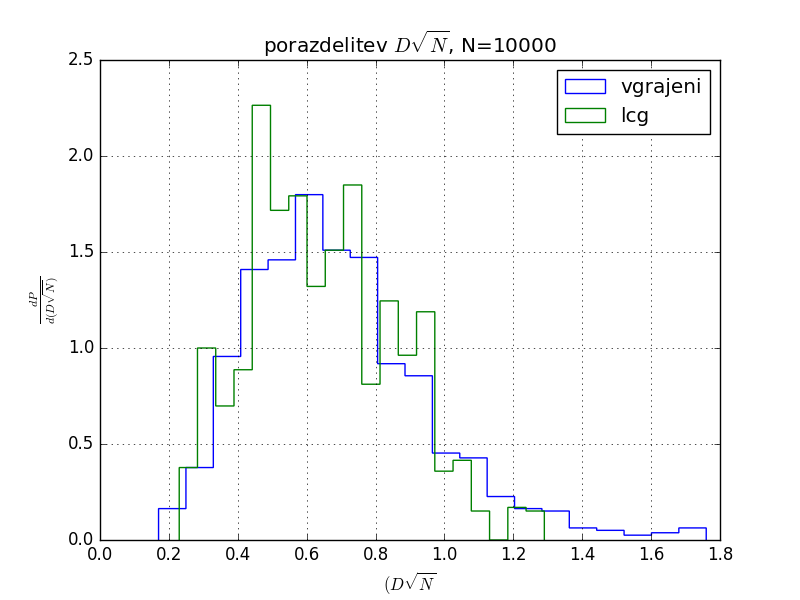
\includegraphics[scale=0.4]{slike/potazdelitev_DsqrtN_10000.png}
%\caption{first figure}
\end{minipage}\hfill

\caption{Porazdelitev $\chi^2$ obeh generatorjev v odvisnosti od števila generiranih številk. Oblike sta podobni, le da ima \textit{lcg} generator nekaj izrazitih vrhov.}
\end{figure}

Iz enačbe \ref{enacba-ks} dobimo za naš primer naslednje mejne vrednosti $D\sqrt{N}$:

\begin{table}[!h]
\begin{center}
\begin{tabular}{|l|l|l|l|}
\hline
stopnja tveganja $\alpha$ & $0.01$ & $0.5$ & $0.99$ \\ \hline
$D\sqrt{N}$ & $0.44$ & $0.83$ & $1.63$ \\ \hline
\end{tabular}
\end{center}
\end{table}



\begin{table}[!h]
\begin{center}
\begin{tabular}{|l|l|l|l|l|}
\hline
generator & \multicolumn{2}{c|}{\textit{lcg}} &  \multicolumn{2}{c|}{vgrajeni}  \\ \hline
$N$ & povprečni $D\sqrt{N}$ & variacija $D\sqrt{N}$ & povprečni $D\sqrt{N}$ & variacija $D\sqrt{N}$ \\  \hline
$100$ & $0.68$ & $0.26$ & $0.70$ & $0.28$ \\ \hline
$1000$ & $0.70$ & $0.26$ & $0.66$ & $0.24$ \\ \hline
$10000$ & $0.69$ & $0.27$ & $0.66$ & $0.23$ \\ \hline
\end{tabular}
\end{center}
\caption{Tako, kot pri testu $\chi^2$, imamo tokrat vrednosti $D\sqrt{N}$, porazdeljene okoli mejne vrednosti  za stopnjo tveganja $\alpha=50\%$. Tudi tokrat je variacija pričakovane vrednosti velika. Vzrok velike variacije (ist lahko sklepamo za veliko variacijo pri testu $\chi^2$) in velike $50\%$ stopnje tveganja nam, pove, da sta generatorja sprejemljiva in dejansko generirata naključne številke. }
\end{table}

\pagebreak

\subsection{Dvodimenzionalna porazdelitev}


\begin{figure}[h]
\noindent\makebox[\textwidth][l]{%
\hspace{-\dimexpr\oddsidemargin+1in}%

\begin{minipage}[t]{0.5\paperwidth}
\begin{flushleft}

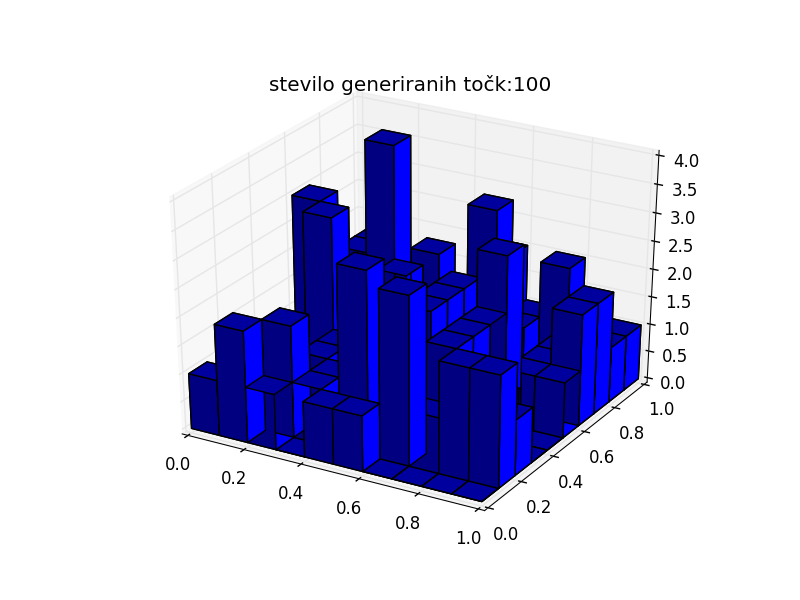
\includegraphics[scale=0.5]{slike/porazdelitev2D_N_100.png}
\hspace{\fill}
\end{flushleft}
\end{minipage}
\begin{minipage}[t]{0.5\paperwidth}
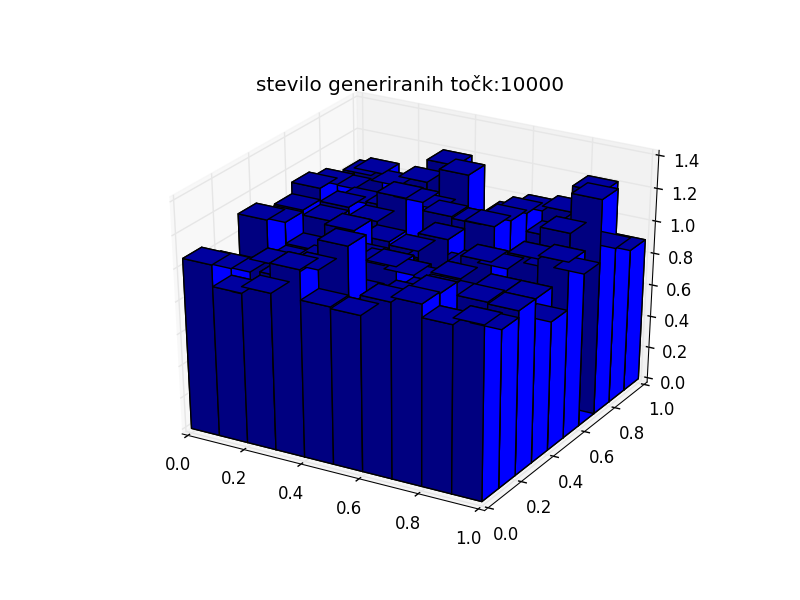
\includegraphics[scale=0.5]{slike/porazdelitev2D_N_10000.png}
\end{minipage}%
}
\caption{Porazdelitev naključnih številk v dveh dimenzijah. Ponovno se lepo vidi, da z večanjem generiranih števil, se porazdelitev približuje konstantni vrednosti.}
\end{figure}

Kaj pa nam pove test $\chi^2$. Sedaj imamo $10*10$ točk, ki jih primerjamo, oz $100-1$ prostostnih stopenj. Iz tabel sledijo mejne vrednosti $\chi^2$:

\begin{table}[!h]
\begin{center}
\begin{tabular}{|l|l|l|l|}
\hline
stopnja tveganja $\alpha$ & $0.01$ & $0.5$ & $0.99$ \\ \hline
$\chi^2$ & $69.23$ & $98.33$ & $134.64$ \\ \hline
\end{tabular}
\end{center}
\end{table}


\begin{table}[!h]
\begin{center}
\begin{tabular}{|l|l|l|}
\hline

$N$ & povprečni $\chi^2$ & variacija $\chi^2$  \\  \hline
$1000$ & $99.01$ & $14.06$ \\ \hline
$10000$ & $99.05$ & $14.11$  \\ \hline
$100000$ & $98.29$ & $14.54$  \\ \hline
\end{tabular}
\end{center}
\caption{Ponovno rezultati testa $\chi^2$ niso presenetljivi. Tudi tokrat povprečna vrednost $\chi^2$ zavzema mejno vrednost pri pričakovani vrednosti $50\%$. Tokrat so variacije približno štirikrat manjše. }
\end{table}








\section{Sevanje v prostoru}
\subsection{Naključna smer v prostoru}
Smer v prostoru najpreprosteje opišemo s sfernima kotoma $\phi$ in $\theta$. Za prehod iz kartezičnih v sferične koordinate moramo upoštevati še "Jacobija":

\begin{equation}
\frac{dP}{dx dy dz} = \frac{dP}{dr d\theta d\phi} r^2 \sin\theta = const.
\end{equation}
Ker nas zanima samo smer izsevanih fotonov, lahko radialno komponento zanemarimo. Z upoštevanjem tega, ter normalizacijo verjetnostne funkcije po prostoru dobimo:
\begin{equation}
\frac{d^2P}{d(\cos\theta) d\phi} =\frac{1}{4 \pi}
\end{equation}

Kot $\phi$ zavzema vrednosti med $0$ in $2 \pi$, ter zaradi preproste zveze v zgornji enačbi vidimo:
\begin{equation}
\frac{dP}{ d\phi} =\frac{1}{2 \pi}
\end{equation}
Za kot $\theta$ potem velja:
\begin{equation}
\frac{dP}{d(\cos\theta)} =\frac{1}{2}
\end{equation}
Iz zgornjih enačb imamo naslednji porazdelitvi kotov:
\begin{equation}
\begin{aligned}
\phi=&2 \pi u \\
\theta =& \arccos(2v-1)
\end{aligned}
\end{equation}
kjer sta $u$, $v$ porazdeljena enakomerno med $0$ in $1$. Porazdelitev po kotu $\phi$ je trivialna (enakomerna med $0$ in $2\pi$), zato si oglejmo porazdelitev po kotu $\theta$.



\begin{figure}[h]
\noindent\makebox[\textwidth][l]{%
\hspace{-\dimexpr\oddsidemargin+1in}%

\begin{minipage}[t]{0.5\paperwidth}
\begin{flushleft}

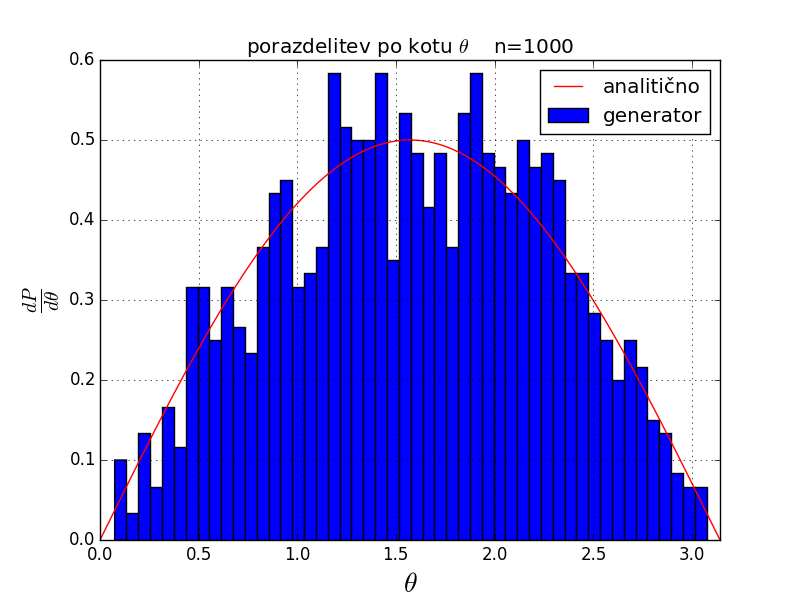
\includegraphics[scale=0.5]{slike/porazdelitev_thetan_1000.png}
%\caption{Nelinearno prilagajanje $I=I_0 [\exp{\frac{U}{U_a}}- \exp{-\frac{U}{U_b}}]$.}
\hspace{\fill}
\end{flushleft}
\end{minipage}
\begin{minipage}[t]{0.5\paperwidth}
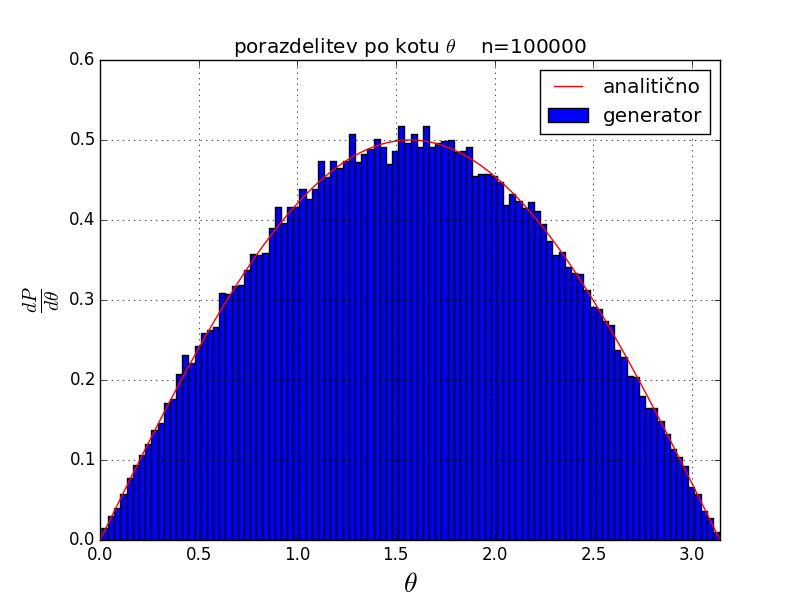
\includegraphics[scale=0.5]{slike/porazdelitev_thetan_100000.png}
%\caption{Nelinearno prilagajanje s premikom napetosti.}
\end{minipage}%
}
\caption{Porazdelitev kota $\theta$, pri naključni smeri v prostori. Na levem grafu imamo $1000$ naključnih smeri in $50$ razdelčnov, na desni pa $10^{5}$ naključnih smeri ter 100 razdelčkov. Rdeča krivulja, je analitična rešitev. Z dovolj veliko številom naključnih smeri se izbrane smeri približujejo analitični rešitvi.}
\end{figure}


Primerjajmo kvaliteto našega generatorja naključnih smeri številčno. Za primerjavo vzemimo računanje nekaj osnovnih momentov. Moment se matematično izračuna:
\begin{equation}
<M>=A\int_0^{\pi} d \theta \int_0^{2 \pi} d \phi M(\theta, \phi) \sin \theta d\theta d \phi 
\end{equation}
kjer je $M$ funkcija našega momenta ter $A$ normalizacijska konstanta. V našem primeru je normalizacijska konstanta enaka $\frac{1}{4 \pi}$. Za numerični izračun momenta funkcije, se zgornja enačba preoblikuje v:
\begin{equation}
<M>=\frac{1}{N} \sum_{i=1}^N M(x_i)\rho(x_i)
\end{equation}
kjer je $M$ funkcija momenta, ter $\rho$ normirana porazdelitvena funkcija. 

\begin{table}[h]
\begin{center}
\begin{tabular}{|c|c|c|}
\hline
moment & analitična vrednost & generator \\ \hline
$<\theta>$ & $\pi /2$ & 1.7530 \\ \hline
$<\cos\theta>$ & $0$ & -0.0017 \\ \hline
$<\phi>$ & $\pi=3.1417$ & 3.1561 \\ \hline
$<\cos \phi>$ & $0$ & -0.0016 \\ \hline
$<\sin \theta>$ & $\pi/4=0.7854$ & 0.7848 \\ \hline
$<Y_2^0>$ & $0$ & 0.0013 \\ \hline
$<\cos^2 \theta>$ & $1/3$ & 0.3338 \\ \hline
$<\cos^2 \phi>$ & $1/5$ & 0.4992 \\ \hline
\end{tabular}
\label{}
\end{center}
\end{table}


\pagebreak

\subsection{Sevanje dipola}
Fotoni so pri dipolnem sevanju prostorsko porazdeljeni: 
\begin{equation}
\frac{dP}{d \Omega}=A \sin^2 \theta
\end{equation}
Iz normalizacije sledi vrednost normalizacijske konstante $A=\frac{3}{8 \pi}$. Trivialno se vidi, da je kot $\phi$ enakomerno porazdeljen med $0$ in $2\pi$. Za določitev porazdelitve po kotu $\theta$, najprej zgornjo porazdelitev transformiramo v kumulativno porazdelitev:
\begin{equation}
\begin{aligned}
F(\theta)=u=&\frac{3}{8\pi}\int_0^{2\pi} \int_0^\theta  \sin^2 \theta' \sin \theta' d\theta' d\phi' \\
&\\
u=&\frac{3}{8\pi} \left[\frac{\cos^3 \theta}{3} -\cos \theta +\frac{2}{3} \right]
\end{aligned}
\end{equation}
Spremenljivka u je sedaj enakomerno porazdeljena med $0$ in $1$, ter sedaj poiščemo inverz zgornje funkcije oz. izpostavimo $\theta$. Ker tega ne moremo rešiti analitično, bomo inverz poiskali s pomočjo bisekcije. 

\begin{figure}[h]
\noindent\makebox[\textwidth][l]{%
\hspace{-\dimexpr\oddsidemargin+1in}%

\begin{minipage}[t]{0.5\paperwidth}
\begin{flushleft}

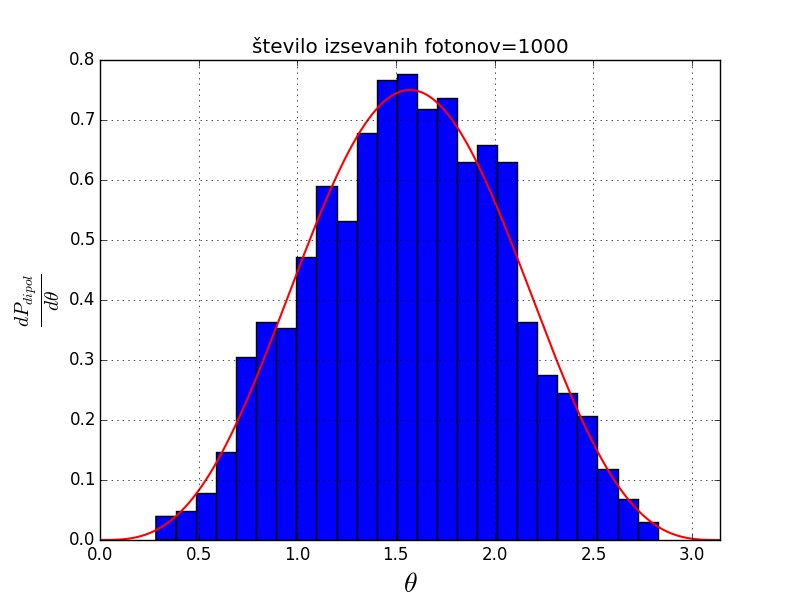
\includegraphics[scale=0.5]{slike/dipol_theta_1000.png}
%\caption{Nelinearno prilagajanje $I=I_0 [\exp{\frac{U}{U_a}}- \exp{-\frac{U}{U_b}}]$.}
\hspace{\fill}
\end{flushleft}
\end{minipage}
\begin{minipage}[t]{0.5\paperwidth}
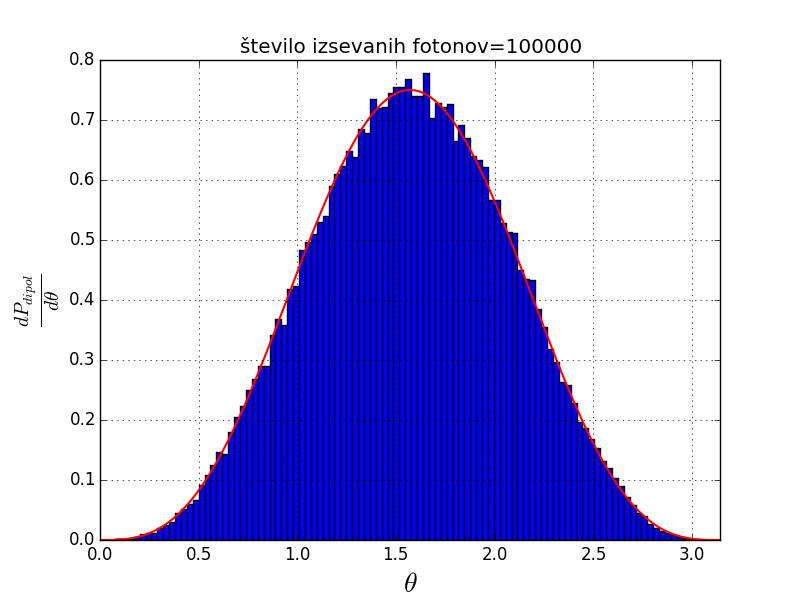
\includegraphics[scale=0.5]{slike/dipol_theta_100000.png}
%\caption{Nelinearno prilagajanje s premikom napetosti.}
\end{minipage}%
}
\caption{Porazdelitev  smeri izsevanih fotonov po kotu $\theta$ (za kot $\phi$ je porazdelitev enakomerna med $0$ in $2qpi$). Na levem grafu imamo $1000$ fotonov in $25$ razdelčnov, na desni pa $10^{5}$ fotonov ter 100 razdelčkov. Rdeča krivulja, je analitična rešitev: $\frac{d P_{dipol}}{d \theta}=\frac{3}{4} \sin^3 \theta$.}
\end{figure}
Tako kot v prejšnjem poglavju si oglejmo nekaj osnovnih momentov:


\begin{table}[h]
\begin{center}
\begin{tabular}{|c|c|c|}
\hline
moment & analitična vrednost & generator \\ \hline
$<\theta>$ & $\pi /2=1.5708$ & 1.5729 \\ \hline
$<\cos\theta>$ & $0$ & -0.0020 \\ \hline
$<\phi>$ & $\pi=3.1417$ & 3.1561 \\ \hline
$<\cos \phi>$ & $0$ & -0.0016 \\ \hline
$<\sin \theta>$ & $\frac{9}{32} \pi=0.8836$ & 0.8840 \\ \hline
$<Y_2^0>$ & $\frac{1}{2\sqrt{2 \pi}}=0.1262$ & -0.1267 \\ \hline
$<\cos^2 \theta>$ & $1/5$ & 0.1995 \\ \hline
$<\cos^2 \phi>$ & $1/2$ & 0.4992 \\ \hline
\end{tabular}
\label{}
\caption{Za računanje momentov smo uporabili $10^{5}$ fotonov in $100$ predalčkov pri risanju histograma.}
\end{center}
\end{table}
Oglejmo si kako hitro konvergirajo izračunane vrednosti k analitični vrednosti.

\begin{figure}[h]
\begin{center}
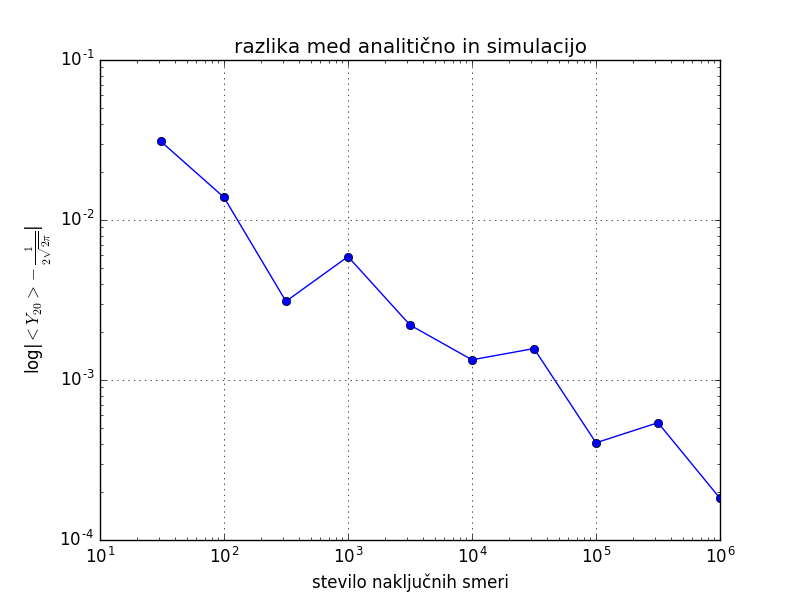
\includegraphics[scale=0.4]{slike/hitrost_variacije.png}
\end{center}
\caption{Hitrost približevanja analitični vrednosti. Na obeh skalah imamo logaritemsko skalo in lahko sklepamo, da se s povečevanjem števila števk oz. fotonov linearno povečujemo veljavna mesta izračunani vrednosti. }
\end{figure}



\section{Box-Mullerjev generator in konvolucijski generator}
V prvi nalogi smo testirali enakomerno porazdeljene naključne številke. Sedaj bomo testirali dva generatorja naključnih števil, ki so porazdeljene po Gaussu. Prvi generator je \textit{Box_mullerjev} generator, ki generira števke $x$ z uporabo enakomerno porazdeljene naključne spremenljivke $x_1$ in $x_2$ ter enačbe:
\begin{equation}
\frac{dP}{dx} = \sqrt{-2 \log{x_1}} \cos(2 \pi x_2)
\end{equation}
Drugi generator se naslanja na centralni limitni izrek, ki pravi, da je vsota $N$ enakomerno porazdeljenih naključnih spremenljivk enakih normalni porazdelitvi. V našem generatorju bo $N=12$, ker pa se vrh premakne za $\frac{N}{2}$, ga je potrebno še prej prestaviti v izhodišče. Širino predpostavimo, da je neodvisna od in je enaka $1$. za večje $N$-je je širina odvisna od $N$.

\begin{figure}[!t]
\noindent\makebox[\textwidth][l]{%
\hspace{-\dimexpr\oddsidemargin+1in}%

\begin{minipage}[t]{0.5\paperwidth}
\begin{flushleft}

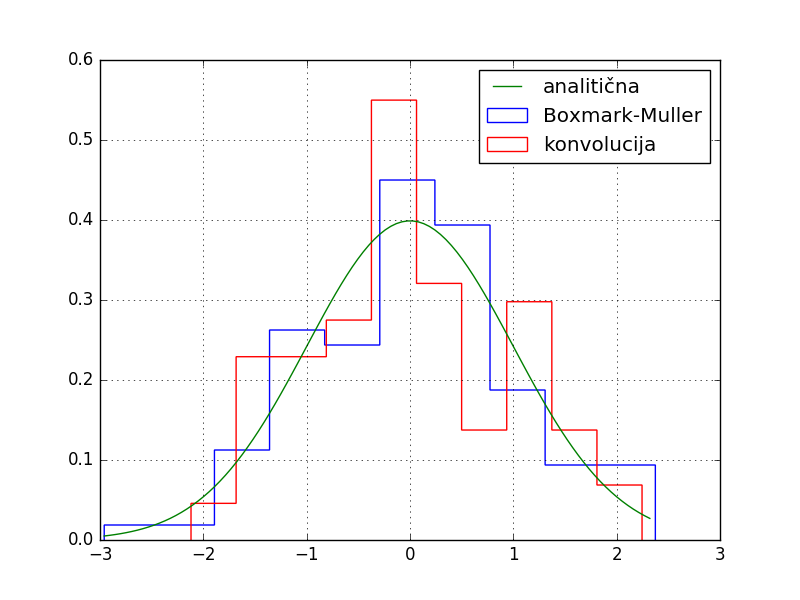
\includegraphics[scale=0.5]{slike/boxmark_konvolucija_gauss_n_100.png}
\hspace{\fill}
\end{flushleft}
\end{minipage}
\begin{minipage}[t]{0.5\paperwidth}
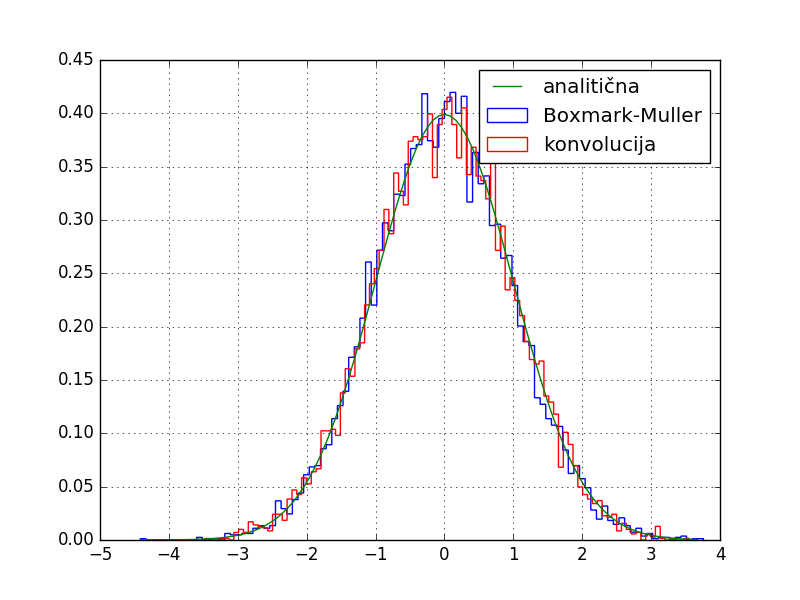
\includegraphics[scale=0.5]{slike/boxmark_konvolucija_gauss_n_10000.png}
\end{minipage}%
}
\caption{Primerjava porazdelitev različnih generatorjev normalno porazdeljenih števil. Na desni imamo $10000$ generiranih številk in $100$ predalčkov, medtem, ko je na levi strani $100$ števk in $10$ predalčkov. Inženirsko lahko rečemo, da generatorja generirata dobro porazdelitev številk.}
\end{figure}

Še mejne vrednosti za testa $\chi^2$ in test Kolmogorov-Smirnov:



\begin{table}[!h]
\begin{center}
\begin{tabular}{|l|l|l|l|}
\hline
$\alpha$ & $0.01$ & $0.5$ & $0.99$ \\ \hline
$m=49$ $\chi^2$ & $28.9$ & $48.3$ & $74.9$ \\ \hline
Kolmogorov-Smirnov & $0.44$ & $0.83$ & $1.63$ \\ \hline
\end{tabular}
\end{center}
\end{table}

\begin{table}[!h]
\begin{center}
\begin{tabular}{|l|l|l|l|l|}
\hline
generator & \multicolumn{2}{c|}{Konvolucija} &  \multicolumn{2}{c|}{Box-Muller}  \\ \hline
$N$ & povprečni $\chi^2$ & variacija $\chi^2$ & povprečni $\chi^2$ & variacija $\chi^2$ \\  \hline
$1000$ & $46.88$ & $12.26$ & $59.96$ & $16.68$ \\ \hline
$10000$ & $49.56$ & $10.62$ & $62.67$ & $51.61$ \\ \hline
$100000$ & $83.37$ & $13.45$ & $62.23$ & $32.45$ \\ \hline
\end{tabular}
\end{center}
\end{table}



\begin{table}[!h]
\begin{center}
\begin{tabular}{|l|l|l|l|l|}
\hline
generator & \multicolumn{2}{c|}{konvolucija} &  \multicolumn{2}{c|}{Box-Muller}  \\ \hline
$N$ & povprečni $D\sqrt{N}$ & variacija $D\sqrt{N}$ & povprečni $D\sqrt{N}$ & variacija $D\sqrt{N}$ \\  \hline
$1000$ & $0.77$ & $027$ & $0.76$ & $0.27$ \\ \hline
$10000$ & $0.81$ & $0.24$ & $0.71$ & $0.20$ \\ \hline
$100000$ & $1.23$ & $0.23$ & $0.69$ & $0.25$ \\ \hline
\end{tabular}
\end{center}
\end{table}

Iz testiranja opazimo, da je Box-Mullerjev test boljši od konvolucijskega. Lahko da k temu rezultatu vpliva dejstvo, da pri konvoluciji imamo območje števk med $0$ in $12$, medtem ko ima prava porazdelitev vrednosti tudi izven tega intervala.




\section{Časi oddaj nalog}



Poglejmo si še kako so v preteklih letih oddajali domače naloge pri predmetu modelska analiza. Iz kumulativne porazdelitve oddaj nalog opazimo, da je večina nalog že oddanih pred rokom. Opazimo tudi dve izrazite stopnici pri vseh letih, ena pri okoli $-100min$, druga pa pri okoli $0min$.

\begin{figure}[h]
\begin{center}
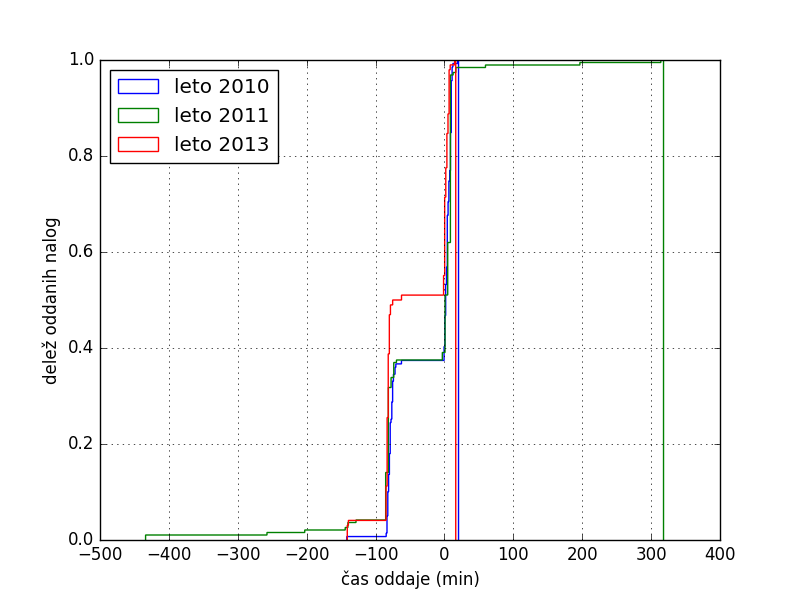
\includegraphics[scale=0.5]{slike/kumulativna_oddaje_nalog_posamezna_leta.png}
\end{center}
\caption{Kumulativna porazdelitev oddanih nalog po posameznih letih. }
\end{figure}

Ker je funkcija $erf(x)$ v grobem približku podobna stopnici, predpostavimo, da je čas oddaje porazdeljen Gaussovsko. Testirali bomo vsa leta skupaj, predpostavimo, da so vsa leta oddajali pod enakimi pogoji. Najprej iz dane porazdelitve prilagajajmo normalno funkcijo, da dobimo vrh in širino časa oddajanja. Dobimo: čas $-30.5min$ in širino $57.7min$.


\begin{figure}[h]
\begin{center}
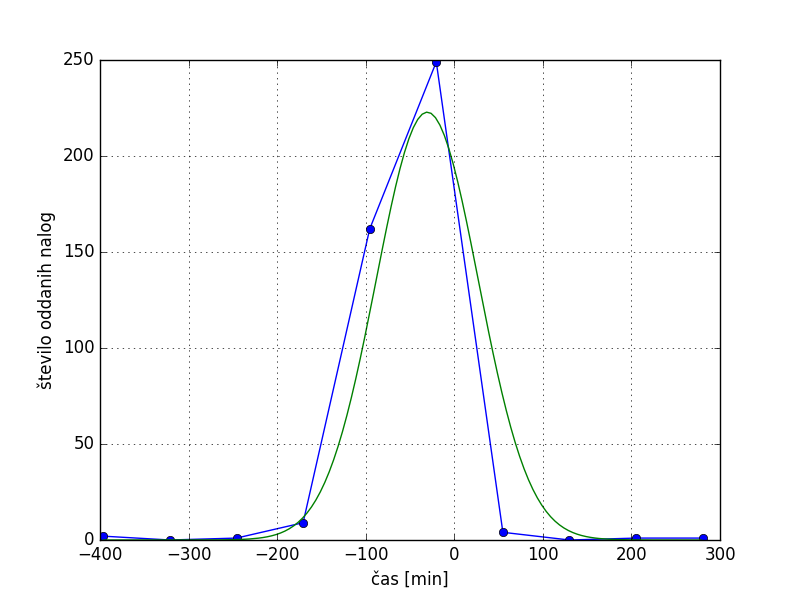
\includegraphics[scale=0.5]{slike/oddaje_nalog_gauss.png}
\end{center}
\caption{POrazdelitev oddanih nalog in njihova Gaussova prilagoditev. Kljub temu, da je prilagajanje izgleda dobro, testa $\chi^2$ in Kolmogorov ne prestane, saj so vrednosti občutno prevelike: $\chi^2=9217901$ in $D\sqrt{N}=3.54$. }
\end{figure}


%----------------------------------------------------------------------













\end{document}
